\documentclass[aspectratio=169]{beamer}
\geometry{paperwidth=320mm,paperheight=180mm}
\usepackage{fontspec}
\setmainfont[Path=fonts/,FontIndex=7,BoldFont=AvenirNext.ttc,BoldFeatures={FontIndex=2},ItalicFont=AvenirNext.ttc,ItalicFeatures={FontIndex=4},BoldItalicFont=AvenirNext.ttc,BoldItalicFeatures={FontIndex=3}]{AvenirNext.ttc}
\setsansfont[Path=fonts/,FontIndex=7,BoldFont=AvenirNext.ttc,BoldFeatures={FontIndex=2},ItalicFont=AvenirNext.ttc,ItalicFeatures={FontIndex=4},BoldItalicFont=AvenirNext.ttc,BoldItalicFeatures={FontIndex=3}]{AvenirNext.ttc}
\newfontfamily\heavy[Path=fonts/,FontIndex=2]{AvenirNext.ttc}
\setmonofont[Path=fonts/,BoldFont=JetBrainsMono-Bold.ttf,ItalicFont=JetBrainsMono-Italic.ttf,Contextuals=NoAlternate,Ligatures=NoCommon]{JetBrainsMono-Regular.ttf}
\usepackage{xcolor,graphicx,tikz,booktabs,tabularx,listings,amsmath}
\usetikzlibrary{arrows.meta,positioning}
\definecolor{paper}{HTML}{FFFFFF}
\definecolor{ink}{HTML}{252525}
\definecolor{teal}{HTML}{252525}
\definecolor{orange}{HTML}{777777}
\definecolor{wash}{HTML}{EAEAEA}
\definecolor{quiet}{HTML}{666666}
\definecolor{lightink}{HTML}{D0D0D0}
\definecolor{codepaper}{HTML}{F6F6F4}
\lstset{language=Python,basicstyle=\ttfamily\fontsize{9.5}{13}\selectfont\color{ink},keywordstyle=\bfseries\color{ink},commentstyle=\itshape\color{quiet},stringstyle=\color{ink},showstringspaces=false,columns=fullflexible,keepspaces=true,breaklines=true,breakatwhitespace=true,numbers=none,upquote=true,aboveskip=8pt,belowskip=6pt}
\hyphenpenalty=4000
\emergencystretch=3em
% The same two-line navigation and fine rule as the reference, without a candy motif.
\newcommand{\guideheader}[2]{\begin{tikzpicture}[remember picture,overlay]
\node[anchor=north west,inner sep=0,text width=176mm] at ([xshift=16mm,yshift=-7mm]current page.north west) {\fontsize{8.5}{10}\selectfont\color{quiet}#1};
\node[anchor=north west,inner sep=0,text width=176mm] at ([xshift=16mm,yshift=-11.5mm]current page.north west) {\heavy\fontsize{10}{12}\selectfont\color{ink}#2};
\draw[lightink,line width=.4pt] ([xshift=16mm,yshift=-17mm]current page.north west)--([xshift=192mm,yshift=-17mm]current page.north west);
\end{tikzpicture}}

\usepackage{colortbl}
\usetikzlibrary{fit}
\newsavebox{\codebox}
\setbeamercolor{normal text}{fg=ink,bg=paper}
\setbeamertemplate{navigation symbols}{}\setbeamertemplate{footline}{}\setbeamertemplate{headline}{}
\begin{document}
\begin{frame}[plain,fragile]\begin{tikzpicture}[remember picture,overlay,x=1cm,y=1cm]\begin{scope}[shift={(current page.south west)}]
\node[anchor=north west,inner sep=0pt,text width=29cm,align=left,text=teal,font=\fontsize{16}{\dimexpr16pt*6/5\relax}\selectfont] at (1.5,16.5) {\heavy LESSON 5};
\node[anchor=north west,inner sep=0pt,text width=29cm,align=left,text=ink,font=\fontsize{46}{\dimexpr46pt*6/5\relax}\selectfont] at (1.5,14.4) {\heavy Hoof, Paper,\\Scissors};
\node[anchor=north west,inner sep=0pt,text width=29cm,align=left,text=quiet,font=\fontsize{22}{\dimexpr22pt*6/5\relax}\selectfont] at (1.5,9.3) {Choose when to switch};
\node[anchor=south,inner sep=0] at (16,2.3) {
\includegraphics[width=27cm,height=6cm,keepaspectratio]{assets/cover.png}};\node[anchor=west,inner sep=0] at (1.5,1) {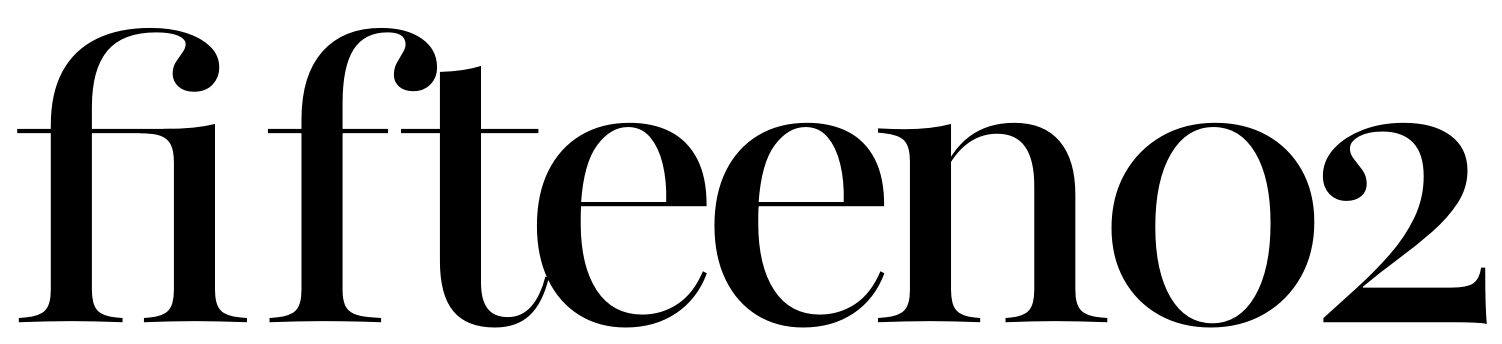
\includegraphics[width=3.8cm]{assets/logo.png}};\node[anchor=east,inner sep=0] at (30.5,1) {
\includegraphics[width=5.5cm]{assets/julians-pathfinder-monochrome.pdf}};
\node[anchor=north west,inner sep=0pt,text width=1cm,align=left,text=quiet,font=\fontsize{11}{\dimexpr11pt*6/5\relax}\selectfont] at (15.8,0.8) {\insertframenumber};
\node[anchor=north west,inner sep=0pt,text width=12cm,align=left,text=ink,font=\fontsize{14}{\dimexpr14pt*6/5\relax}\selectfont] at (18,16.5) {\href{https://colab.research.google.com/github/fifteen02/julians-pathfinder/blob/main/Lesson\%205/lesson.ipynb}{\underline{Open this lesson in Google Colab}}};
\end{scope}\end{tikzpicture}
\end{frame}

\begin{frame}[plain,fragile]\begin{tikzpicture}[remember picture,overlay,x=1cm,y=1cm]\begin{scope}[shift={(current page.south west)}]
\node[anchor=north west,inner sep=0pt,text width=29cm,align=left,text=quiet,font=\fontsize{13}{\dimexpr13pt*6/5\relax}\selectfont] at (1.5,16.9) {\heavy LESSON 5 / TODAY};
\node[anchor=north west,inner sep=0pt,text width=1cm,align=left,text=quiet,font=\fontsize{11}{\dimexpr11pt*6/5\relax}\selectfont] at (30,0.8) {\insertframenumber};
\node[anchor=north west,inner sep=0pt,text width=29cm,align=left,text=quiet,font=\fontsize{18}{\dimexpr18pt*6/5\relax}\selectfont] at (1.5,15.4) {\heavy MAIN IDEA};
\node[anchor=north west,inner sep=0pt,text width=29cm,align=left,text=ink,font=\fontsize{40}{\dimexpr40pt*6/5\relax}\selectfont] at (1.5,14.3) {\heavy Choose when to switch.};
\node(idea)[anchor=north west,inner sep=0pt,text width=28cm,align=left,text=ink,font=\fontsize{24}{\dimexpr24pt*6/5\relax}\selectfont] at (1.5,11.9) {Keep the round, the switches used and the current gesture; at every round, compare staying with switching.};
\node[anchor=north west,inner sep=0pt,text width=28cm,align=left,font=\fontsize{24}{30}\selectfont] at ([yshift=-9mm]idea.south west) {\textbf{You will be able to}\par\smallskip\hangindent=1.1em\hangafter=1\textbullet\ record the round, switches used and ending gesture for each score;\par\hangindent=1.1em\hangafter=1\textbullet\ explain why at most K switches is not the same as exactly K switches;\par\hangindent=1.1em\hangafter=1\textbullet\ fill each round from the previous round by comparing stay and switch.\par};
\end{scope}\end{tikzpicture}
\end{frame}

\begin{frame}[plain,fragile]\begin{tikzpicture}[remember picture,overlay,x=1cm,y=1cm]\begin{scope}[shift={(current page.south west)}]
\node[anchor=north west,inner sep=0pt,text width=29cm,align=left,text=quiet,font=\fontsize{13}{\dimexpr13pt*6/5\relax}\selectfont] at (1.5,16.9) {\heavy LESSON 5 / L5-01 / QUESTION};
\node[anchor=north west,inner sep=0pt,text width=1cm,align=left,text=quiet,font=\fontsize{11}{\dimexpr11pt*6/5\relax}\selectfont] at (30,0.8) {\insertframenumber};
\node[anchor=north west,inner sep=0pt,text width=29cm,align=left,text=ink,font=\fontsize{34}{\dimexpr34pt*6/5\relax}\selectfont] at (1.5,15.4) {\heavy Which gesture wins?};
\node(body)[anchor=north west,inner sep=0pt,text width=29cm,align=left,text=ink,font=\fontsize{22}{\dimexpr22pt*6/5\relax}\selectfont] at (1.5,12.4) {H means hoof, P paper and S scissors. H beats S, S beats P, and P beats H. A win scores 1; a draw or loss scores 0. John plays H, H, S, S, P. Fill Bessie's wins in each round when she keeps H throughout, then when she keeps P or S.};
\node(tab)[anchor=north west,inner sep=0,text width=29cm] at ([yshift=-8mm]body.south west) {\begingroup\fontsize{20}{24}\selectfont\setlength{\tabcolsep}{5pt}\setlength{\arrayrulewidth}{.5pt}\arrayrulecolor{quiet}\renewcommand{\arraystretch}{1}\begin{tabularx}{\linewidth}{|>{\raggedright\arraybackslash}p{34mm}|>{\centering\arraybackslash}X|>{\centering\arraybackslash}X|>{\centering\arraybackslash}X|>{\centering\arraybackslash}X|>{\centering\arraybackslash}X|}\hline
\rowcolor{wash}\rule[-2.6mm]{0pt}{8mm}\textbf{Round} & \textbf{0} & \textbf{1} & \textbf{2} & \textbf{3} & \textbf{4}\\\hline
\rule[-3.4mm]{0pt}{11.5mm}John & H & H & S & S & P\\\hline
\rule[-3.4mm]{0pt}{11.5mm}Keep H &  &  &  &  & \\\hline
\rule[-3.4mm]{0pt}{11.5mm}Keep P &  &  &  &  & \\\hline
\rule[-3.4mm]{0pt}{11.5mm}Keep S &  &  &  &  & \\\hline
\end{tabularx}\endgroup};
\end{scope}\end{tikzpicture}
\end{frame}

\begin{frame}[plain,fragile]\begin{tikzpicture}[remember picture,overlay,x=1cm,y=1cm]\begin{scope}[shift={(current page.south west)}]
\node[anchor=north west,inner sep=0pt,text width=29cm,align=left,text=quiet,font=\fontsize{13}{\dimexpr13pt*6/5\relax}\selectfont] at (1.5,16.9) {\heavy LESSON 5 / L5-01 / ANSWER};
\node[anchor=north west,inner sep=0pt,text width=1cm,align=left,text=quiet,font=\fontsize{11}{\dimexpr11pt*6/5\relax}\selectfont] at (30,0.8) {\insertframenumber};
\node[anchor=north west,inner sep=0pt,text width=29cm,align=left,text=ink,font=\fontsize{34}{\dimexpr34pt*6/5\relax}\selectfont] at (1.5,15.4) {\heavy Which gesture wins?};
\node(body)[anchor=north west,inner sep=0pt,text width=29cm,align=left,text=ink,font=\fontsize{22}{\dimexpr22pt*6/5\relax}\selectfont] at (1.5,12.4) {Keeping H wins twice, against the two S rounds. Keeping P wins twice, against the two H rounds. Keeping S wins once, against P. Draws and losses each contribute zero wins.};
\node(tab)[anchor=north west,inner sep=0,text width=29cm] at ([yshift=-8mm]body.south west) {\begingroup\fontsize{20}{24}\selectfont\setlength{\tabcolsep}{5pt}\setlength{\arrayrulewidth}{.5pt}\arrayrulecolor{quiet}\renewcommand{\arraystretch}{1}\begin{tabularx}{\linewidth}{|>{\raggedright\arraybackslash}p{34mm}|>{\centering\arraybackslash}X|>{\centering\arraybackslash}X|>{\centering\arraybackslash}X|>{\centering\arraybackslash}X|>{\centering\arraybackslash}X|}\hline
\rowcolor{wash}\rule[-2.6mm]{0pt}{8mm}\textbf{Round} & \textbf{0} & \textbf{1} & \textbf{2} & \textbf{3} & \textbf{4}\\\hline
\rule[-3.4mm]{0pt}{11.5mm}John & H & H & S & S & P\\\hline
\rule[-3.4mm]{0pt}{11.5mm}Keep H & 0 & 0 & 1 & 1 & 0\\\hline
\rule[-3.4mm]{0pt}{11.5mm}Keep P & 1 & 1 & 0 & 0 & 0\\\hline
\rule[-3.4mm]{0pt}{11.5mm}Keep S & 0 & 0 & 0 & 0 & 1\\\hline
\end{tabularx}\endgroup};
\end{scope}\end{tikzpicture}
\end{frame}

\begin{frame}[plain,fragile]\begin{tikzpicture}[remember picture,overlay,x=1cm,y=1cm]\begin{scope}[shift={(current page.south west)}]
\node[anchor=north west,inner sep=0pt,text width=29cm,align=left,text=quiet,font=\fontsize{13}{\dimexpr13pt*6/5\relax}\selectfont] at (1.5,16.9) {\heavy LESSON 5 / L5-02 / QUESTION};
\node[anchor=north west,inner sep=0pt,text width=1cm,align=left,text=quiet,font=\fontsize{11}{\dimexpr11pt*6/5\relax}\selectfont] at (30,0.8) {\insertframenumber};
\node[anchor=north west,inner sep=0pt,text width=29cm,align=left,text=ink,font=\fontsize{34}{\dimexpr34pt*6/5\relax}\selectfont] at (1.5,15.4) {\heavy Zero switches is already a useful case};
\node(body)[anchor=north west,inner sep=0pt,text width=29cm,align=left,text=ink,font=\fontsize{25}{\dimexpr25pt*6/5\relax}\selectfont] at (1.5,12.4) {With no switches allowed, how would you solve the whole game? What answer do you get for H, H, S, S, P?};
\node[anchor=south,inner sep=0] at (16,2.1) {
\includegraphics[width=24cm,height=5.7cm,keepaspectratio]{assets/slides/gestures.png}};
\node[anchor=north west,inner sep=0pt,text width=28cm,align=left,text=quiet,font=\fontsize{17}{\dimexpr17pt*6/5\relax}\selectfont] at (1.5,1.45) {Think on your own first. Then compare your reasoning with a partner.};
\end{scope}\end{tikzpicture}
\end{frame}

\begin{frame}[plain,fragile]
\begin{tikzpicture}[remember picture,overlay,x=1cm,y=1cm]\begin{scope}[shift={(current page.south west)}]
\node[anchor=north west,inner sep=0pt,text width=29cm,align=left,text=quiet,font=\fontsize{13}{\dimexpr13pt*6/5\relax}\selectfont] at (1.5,16.9) {\heavy LESSON 5 / L5-02 / ANSWER};
\node[anchor=north west,inner sep=0pt,text width=1cm,align=left,text=quiet,font=\fontsize{11}{\dimexpr11pt*6/5\relax}\selectfont] at (30,0.8) {\insertframenumber};
\node[anchor=north west,inner sep=0pt,text width=29cm,align=left,text=ink,font=\fontsize{34}{\dimexpr34pt*6/5\relax}\selectfont] at (1.5,15.4) {\heavy Zero switches is already a useful case};
\node(body)[anchor=north west,inner sep=0pt,text width=29cm,align=left,text=ink,font=\fontsize{25}{\dimexpr25pt*6/5\relax}\selectfont] at (1.5,12.4) {Count the wins for each fixed gesture and take the largest. The answer is 2. Choosing the first gesture is free, so all three fixed strategies are available.};
\node[anchor=north west,inner sep=0pt,text width=28cm,align=left,text=teal,font=\fontsize{21}{\dimexpr21pt*6/5\relax}\selectfont] at (1.5,4.0) {\textbf{Watch for:} Charging a switch for the first gesture incorrectly excludes all zero-switch strategies.};
\end{scope}\end{tikzpicture}
\end{frame}

\begin{frame}[plain,fragile]\begin{tikzpicture}[remember picture,overlay,x=1cm,y=1cm]\begin{scope}[shift={(current page.south west)}]
\node[anchor=north west,inner sep=0pt,text width=29cm,align=left,text=quiet,font=\fontsize{13}{\dimexpr13pt*6/5\relax}\selectfont] at (1.5,16.9) {\heavy LESSON 5 / L5-03 / QUESTION};
\node[anchor=north west,inner sep=0pt,text width=1cm,align=left,text=quiet,font=\fontsize{11}{\dimexpr11pt*6/5\relax}\selectfont] at (30,0.8) {\insertframenumber};
\node[anchor=north west,inner sep=0pt,text width=29cm,align=left,text=ink,font=\fontsize{34}{\dimexpr34pt*6/5\relax}\selectfont] at (1.5,15.4) {\heavy One well-placed switch};
\node(body)[anchor=north west,inner sep=0pt,text width=29cm,align=left,text=ink,font=\fontsize{22}{\dimexpr22pt*6/5\relax}\selectfont] at (1.5,12.4) {John plays H, H, S, S, P. Bessie may choose her first gesture freely and change it at most once between rounds. Find a strategy with four wins. Number rounds from 0 and identify the gap where she changes. Can one change produce five wins?};
\node(tab)[anchor=north west,inner sep=0,text width=29cm] at ([yshift=-8mm]body.south west) {\begingroup\fontsize{22}{26}\selectfont\setlength{\tabcolsep}{5pt}\setlength{\arrayrulewidth}{.5pt}\arrayrulecolor{quiet}\renewcommand{\arraystretch}{1}\begin{tabularx}{\linewidth}{|>{\raggedright\arraybackslash}p{34mm}|>{\centering\arraybackslash}X|>{\centering\arraybackslash}X|>{\centering\arraybackslash}X|>{\centering\arraybackslash}X|>{\centering\arraybackslash}X|}\hline
\rowcolor{wash}\rule[-3mm]{0pt}{9.5mm}\textbf{Round} & \textbf{0} & \textbf{1} & \textbf{2} & \textbf{3} & \textbf{4}\\\hline
\rule[-4.6mm]{0pt}{13.5mm}John & H & H & S & S & P\\\hline
\rule[-4.6mm]{0pt}{13.5mm}Bessie &  &  &  &  & \\\hline
\rule[-4.6mm]{0pt}{13.5mm}Wins &  &  &  &  & \\\hline
\end{tabularx}\endgroup};
\end{scope}\end{tikzpicture}
\end{frame}

\begin{frame}[plain,fragile]\begin{tikzpicture}[remember picture,overlay,x=1cm,y=1cm]\begin{scope}[shift={(current page.south west)}]
\node[anchor=north west,inner sep=0pt,text width=29cm,align=left,text=quiet,font=\fontsize{13}{\dimexpr13pt*6/5\relax}\selectfont] at (1.5,16.9) {\heavy LESSON 5 / L5-03 / ANSWER};
\node[anchor=north west,inner sep=0pt,text width=1cm,align=left,text=quiet,font=\fontsize{11}{\dimexpr11pt*6/5\relax}\selectfont] at (30,0.8) {\insertframenumber};
\node[anchor=north west,inner sep=0pt,text width=29cm,align=left,text=ink,font=\fontsize{34}{\dimexpr34pt*6/5\relax}\selectfont] at (1.5,15.4) {\heavy One well-placed switch};
\node(body)[anchor=north west,inner sep=0pt,text width=29cm,align=left,text=ink,font=\fontsize{23}{\dimexpr23pt*6/5\relax}\selectfont] at (1.5,12.4) {Play P, P, H, H, H. Switch once before round 2 and win four rounds. Winning all five would require P, P, H, H, S, which changes twice. Thus 4 is optimal.};
\node[anchor=north west,inner sep=0,text width=14cm] at ([yshift=-8mm]body.south west) {\begingroup\fontsize{22}{26}\selectfont\setlength{\tabcolsep}{5pt}\setlength{\arrayrulewidth}{.5pt}\arrayrulecolor{quiet}\renewcommand{\arraystretch}{1}\begin{tabularx}{\linewidth}{|>{\raggedright\arraybackslash}p{34mm}|>{\centering\arraybackslash}X|>{\centering\arraybackslash}X|>{\centering\arraybackslash}X|>{\centering\arraybackslash}X|>{\centering\arraybackslash}X|}\hline
\rowcolor{wash}\rule[-3mm]{0pt}{9.5mm}\textbf{Round} & \textbf{0} & \textbf{1} & \textbf{2} & \textbf{3} & \textbf{4}\\\hline
\rule[-4.6mm]{0pt}{13.5mm}John & H & H & S & S & P\\\hline
\rule[-4.6mm]{0pt}{13.5mm}Bessie & P & P & H & H & H\\\hline
\rule[-4.6mm]{0pt}{13.5mm}Wins & 1 & 1 & 1 & 1 & 0\\\hline
\end{tabularx}\endgroup};
\node[anchor=south,inner sep=0] at (24.5,1.8) {
\includegraphics[width=12cm,height=6.8cm,keepaspectratio]{assets/slides/switch.png}};
\end{scope}\end{tikzpicture}
\end{frame}

\begin{frame}[plain,fragile]\begin{tikzpicture}[remember picture,overlay,x=1cm,y=1cm]\begin{scope}[shift={(current page.south west)}]
\node[anchor=north west,inner sep=0pt,text width=29cm,align=left,text=quiet,font=\fontsize{13}{\dimexpr13pt*6/5\relax}\selectfont] at (1.5,16.9) {\heavy LESSON 5 / L5-04 / QUESTION};
\node[anchor=north west,inner sep=0pt,text width=1cm,align=left,text=quiet,font=\fontsize{11}{\dimexpr11pt*6/5\relax}\selectfont] at (30,0.8) {\insertframenumber};
\node[anchor=north west,inner sep=0pt,text width=29cm,align=left,text=ink,font=\fontsize{34}{\dimexpr34pt*6/5\relax}\selectfont] at (1.5,15.4) {\heavy What must the state remember?};
\node(body)[anchor=north west,inner sep=0pt,text width=29cm,align=left,text=ink,font=\fontsize{25}{\dimexpr25pt*6/5\relax}\selectfont] at (1.5,12.4) {Two strategies have processed the same rounds and used one switch, but one ends with H and the other with P. Can their best win counts be merged into one number?};
\node[anchor=north west,inner sep=0pt,text width=28cm,align=left,text=teal,font=\fontsize{22}{\dimexpr22pt*6/5\relax}\selectfont] at (1.5,4.0) {Think on your own first. Then compare your reasoning with a partner.};
\end{scope}\end{tikzpicture}
\end{frame}

\begin{frame}[plain,fragile]
\begin{tikzpicture}[remember picture,overlay,x=1cm,y=1cm]\begin{scope}[shift={(current page.south west)}]
\node[anchor=north west,inner sep=0pt,text width=29cm,align=left,text=quiet,font=\fontsize{13}{\dimexpr13pt*6/5\relax}\selectfont] at (1.5,16.9) {\heavy LESSON 5 / L5-04 / ANSWER};
\node[anchor=north west,inner sep=0pt,text width=1cm,align=left,text=quiet,font=\fontsize{11}{\dimexpr11pt*6/5\relax}\selectfont] at (30,0.8) {\insertframenumber};
\node[anchor=north west,inner sep=0pt,text width=29cm,align=left,text=ink,font=\fontsize{34}{\dimexpr34pt*6/5\relax}\selectfont] at (1.5,15.4) {\heavy What must the state remember?};
\node(body)[anchor=north west,inner sep=0pt,text width=29cm,align=left,text=ink,font=\fontsize{25}{\dimexpr25pt*6/5\relax}\selectfont] at (1.5,12.4) {No. Their current gestures differ, so the next gesture may require a switch in one history but not the other. Record the processed round, switches used and current gesture.};
\node[anchor=north west,inner sep=0pt,text width=28cm,align=left,text=teal,font=\fontsize{21}{\dimexpr21pt*6/5\relax}\selectfont] at (1.5,4.0) {\textbf{Watch for:} A history with more wins can still be unsuitable if it has a different gesture or spent budget.};
\end{scope}\end{tikzpicture}
\end{frame}

\begin{frame}[plain,fragile]\begin{tikzpicture}[remember picture,overlay,x=1cm,y=1cm]\begin{scope}[shift={(current page.south west)}]
\node[anchor=north west,inner sep=0pt,text width=29cm,align=left,text=quiet,font=\fontsize{13}{\dimexpr13pt*6/5\relax}\selectfont] at (1.5,16.9) {\heavy LESSON 5 / L5-05 / QUESTION};
\node[anchor=north west,inner sep=0pt,text width=1cm,align=left,text=quiet,font=\fontsize{11}{\dimexpr11pt*6/5\relax}\selectfont] at (30,0.8) {\insertframenumber};
\node[anchor=north west,inner sep=0pt,text width=29cm,align=left,text=ink,font=\fontsize{34}{\dimexpr34pt*6/5\relax}\selectfont] at (1.5,15.4) {\heavy Recursive choices with a budget};
\node(body)[anchor=north west,inner sep=0pt,text width=29cm,align=left,text=ink,font=\fontsize{20}{\dimexpr20pt*6/5\relax}\selectfont] at (1.5,12.4) {Write hps\_cached(john, budget) using recursion. Its helper knows the next round, switches left and previous gesture. How do you handle the first round without charging a switch?};
\node(sig)[anchor=north west,inner sep=3mm,fill=codepaper,align=left,font=\ttfamily\fontsize{16}{20}\selectfont] at ([yshift=-4mm,xshift=3mm]body.south west) {def hps\_cached(john, budget):\\\hspace*{2.4em}def best(i, left, previous):\\\hspace*{4.8em}return None  \# Replace this\\\hspace*{2.4em}return best(0, budget, '')};
\node(result)[anchor=north west,inner sep=0pt,text width=13.5cm,align=left,text=quiet,font=\fontsize{17}{20}\selectfont] at ([yshift=-4mm,xshift=15.5cm]body.south west) {\textbf{Returns}\par \textbf{hps\_cached(john, budget)}: the most rounds Bessie can win within the switch budget.\par\smallskip \textbf{best(i, left, previous)}: the most further wins from round i, with left switches available and previous as the last gesture.\par\smallskip };
\node(both)[fit=(sig)(result),inner sep=0] {};
\node[anchor=north west,inner sep=0pt,text width=29cm,align=left,text=quiet,font=\fontsize{18}{22}\selectfont] at ([yshift=-3mm,xshift=-3mm]both.south west) {\textbf{Hints.} What does best return when no rounds remain? When does choosing a gesture cost a switch, and when is it free? Which choices are not allowed with the switches left?};
\end{scope}\end{tikzpicture}
\end{frame}

\begin{frame}[plain,fragile]\begin{tikzpicture}[remember picture,overlay,x=1cm,y=1cm]\begin{scope}[shift={(current page.south west)}]
\node[anchor=north west,inner sep=0pt,text width=29cm,align=left,text=quiet,font=\fontsize{13}{\dimexpr13pt*6/5\relax}\selectfont] at (1.5,16.9) {\heavy LESSON 5 / L5-05 / ANSWER};
\node[anchor=north west,inner sep=0pt,text width=1cm,align=left,text=quiet,font=\fontsize{11}{\dimexpr11pt*6/5\relax}\selectfont] at (30,0.8) {\insertframenumber};
\node[anchor=north west,inner sep=0pt,text width=29cm,align=left,text=ink,font=\fontsize{34}{\dimexpr34pt*6/5\relax}\selectfont] at (1.5,15.4) {\heavy Recursive choices with a budget};
\node(body)[anchor=north west,inner sep=0pt,text width=29cm,align=left,text=ink,font=\fontsize{25}{\dimexpr25pt*6/5\relax}\selectfont] at (1.5,12.4) {Try each gesture. Charge one switch only if a previous gesture exists and the new one differs. Reject choices that exceed the remaining budget. Add this round's win to the best continuation.};
\node[anchor=north west,inner sep=0pt,text width=28cm,align=left,text=teal,font=\fontsize{21}{\dimexpr21pt*6/5\relax}\selectfont] at (1.5,4.0) {\textbf{Watch for:} Subtracting a switch on the first round breaks budget-zero cases.};
\end{scope}\end{tikzpicture}
\end{frame}

\begin{frame}[plain,fragile]
\begin{lrbox}{\codebox}\begin{minipage}{791pt}
\begin{lstlisting}[basicstyle=\ttfamily\fontsize{16.0}{17.9}\selectfont\color{ink},numbers=left,numberstyle=\ttfamily\fontsize{10.4}{17.9}\selectfont\color{quiet},numbersep=12pt,xleftmargin=26pt,firstnumber=1,breaklines=false,aboveskip=0pt,belowskip=0pt]
from functools import lru_cache

BEATS = {'H': 'S', 'P': 'H', 'S': 'P'}

def hps_cached(john, budget):
    @lru_cache(None)
    def best(i, left, previous):
        if i == len(john):
            return 0
        answer = 0
        for gesture in 'HPS':
            change = int(previous != '' and gesture != previous)
            if change <= left:
                win = int(BEATS[gesture] == john[i])
                answer = max(answer, win + best(i + 1, left - change, gesture))
        return answer
    return best(0, budget, '')
\end{lstlisting}
\end{minipage}\end{lrbox}
\begin{tikzpicture}[remember picture,overlay,x=1cm,y=1cm]\begin{scope}[shift={(current page.south west)}]
\node[anchor=north west,inner sep=0pt,text width=29cm,align=left,text=quiet,font=\fontsize{13}{\dimexpr13pt*6/5\relax}\selectfont] at (1.5,16.9) {\heavy LESSON 5 / L5-05 / ANSWER: PYTHON};
\node[anchor=north west,inner sep=0pt,text width=1cm,align=left,text=quiet,font=\fontsize{11}{\dimexpr11pt*6/5\relax}\selectfont] at (30,0.8) {\insertframenumber};
\node[anchor=north west,inner sep=0pt,text width=29cm,align=left,text=ink,font=\fontsize{34}{40.8}\selectfont] at (1.5,15.4) {\heavy hps cached};
\node[anchor=north,inner sep=5mm,fill=codepaper] at (16,13.6) {\usebox{\codebox}};
\end{scope}\end{tikzpicture}

\end{frame}

\begin{frame}[plain,fragile]\begin{tikzpicture}[remember picture,overlay,x=1cm,y=1cm]\begin{scope}[shift={(current page.south west)}]
\node[anchor=north west,inner sep=0pt,text width=29cm,align=left,text=quiet,font=\fontsize{13}{\dimexpr13pt*6/5\relax}\selectfont] at (1.5,16.9) {\heavy LESSON 5 / L5-06 / QUESTION};
\node[anchor=north west,inner sep=0pt,text width=1cm,align=left,text=quiet,font=\fontsize{11}{\dimexpr11pt*6/5\relax}\selectfont] at (30,0.8) {\insertframenumber};
\node[anchor=north west,inner sep=0pt,text width=29cm,align=left,text=ink,font=\fontsize{34}{\dimexpr34pt*6/5\relax}\selectfont] at (1.5,15.4) {\heavy Exactly used versus at most allowed};
\node(body)[anchor=north west,inner sep=0pt,text width=29cm,align=left,text=ink,font=\fontsize{22}{\dimexpr22pt*6/5\relax}\selectfont] at (1.5,12.4) {John plays H in round 0. Fill Bessie's scores for each ending gesture H, P and S with exactly zero switches used. Can exactly one switch have been used after just this round? Write a dash for impossible states and explain why a score of 0 would mean something different.};
\node(tab)[anchor=north west,inner sep=0,text width=29cm] at ([yshift=-8mm]body.south west) {\begingroup\fontsize{22}{26}\selectfont\setlength{\tabcolsep}{5pt}\setlength{\arrayrulewidth}{.5pt}\arrayrulecolor{quiet}\renewcommand{\arraystretch}{1}\begin{tabularx}{\linewidth}{|>{\raggedright\arraybackslash}p{68mm}|>{\centering\arraybackslash}X|>{\centering\arraybackslash}X|>{\centering\arraybackslash}X|}\hline
\rowcolor{wash}\rule[-3mm]{0pt}{9.5mm}\textbf{Switches used} & \textbf{End H} & \textbf{End P} & \textbf{End S}\\\hline
\rule[-4.6mm]{0pt}{13.5mm}0 &  &  & \\\hline
\rule[-4.6mm]{0pt}{13.5mm}1 &  &  & \\\hline
\end{tabularx}\endgroup};
\end{scope}\end{tikzpicture}
\end{frame}

\begin{frame}[plain,fragile]\begin{tikzpicture}[remember picture,overlay,x=1cm,y=1cm]\begin{scope}[shift={(current page.south west)}]
\node[anchor=north west,inner sep=0pt,text width=29cm,align=left,text=quiet,font=\fontsize{13}{\dimexpr13pt*6/5\relax}\selectfont] at (1.5,16.9) {\heavy LESSON 5 / L5-06 / ANSWER};
\node[anchor=north west,inner sep=0pt,text width=1cm,align=left,text=quiet,font=\fontsize{11}{\dimexpr11pt*6/5\relax}\selectfont] at (30,0.8) {\insertframenumber};
\node[anchor=north west,inner sep=0pt,text width=29cm,align=left,text=ink,font=\fontsize{34}{\dimexpr34pt*6/5\relax}\selectfont] at (1.5,15.4) {\heavy Exactly used versus at most allowed};
\node(body)[anchor=north west,inner sep=0pt,text width=29cm,align=left,text=ink,font=\fontsize{22}{\dimexpr22pt*6/5\relax}\selectfont] at (1.5,12.4) {For ending gestures H, P, S, the zero-switch scores are [0, 1, 0]. Exactly one switch is impossible after one round. Mark impossible states with negative infinity, not zero.};
\node(tab)[anchor=north west,inner sep=0,text width=29cm] at ([yshift=-8mm]body.south west) {\begingroup\fontsize{22}{26}\selectfont\setlength{\tabcolsep}{5pt}\setlength{\arrayrulewidth}{.5pt}\arrayrulecolor{quiet}\renewcommand{\arraystretch}{1}\begin{tabularx}{\linewidth}{|>{\raggedright\arraybackslash}p{68mm}|>{\centering\arraybackslash}X|>{\centering\arraybackslash}X|>{\centering\arraybackslash}X|}\hline
\rowcolor{wash}\rule[-3mm]{0pt}{9.5mm}\textbf{Switches used} & \textbf{End H} & \textbf{End P} & \textbf{End S}\\\hline
\rule[-4.6mm]{0pt}{13.5mm}0 & 0 & 1 & 0\\\hline
\rule[-4.6mm]{0pt}{13.5mm}1 & impossible & impossible & impossible\\\hline
\end{tabularx}\endgroup};
\end{scope}\end{tikzpicture}
\end{frame}

\begin{frame}[plain,fragile]\begin{tikzpicture}[remember picture,overlay,x=1cm,y=1cm]\begin{scope}[shift={(current page.south west)}]
\node[anchor=north west,inner sep=0pt,text width=29cm,align=left,text=quiet,font=\fontsize{13}{\dimexpr13pt*6/5\relax}\selectfont] at (1.5,16.9) {\heavy LESSON 5 / L5-07 / QUESTION};
\node[anchor=north west,inner sep=0pt,text width=1cm,align=left,text=quiet,font=\fontsize{11}{\dimexpr11pt*6/5\relax}\selectfont] at (30,0.8) {\insertframenumber};
\node[anchor=north west,inner sep=0pt,text width=29cm,align=left,text=ink,font=\fontsize{34}{\dimexpr34pt*6/5\relax}\selectfont] at (1.5,15.4) {\heavy Stay or switch before this round};
\node(body)[anchor=north west,inner sep=0pt,text width=29cm,align=left,text=ink,font=\fontsize{22}{\dimexpr22pt*6/5\relax}\selectfont] at (1.5,12.4) {After John plays H,H, scores for ending H,P,S are [0,2,0] with no switches and [1,1,1] with exactly one. John now plays S. For an ending H with exactly one switch, compare staying with H against changing from P or S. Then fill both new score rows.};
\node(tab)[anchor=north west,inner sep=0,text width=29cm] at ([yshift=-8mm]body.south west) {\begingroup\fontsize{22}{26}\selectfont\setlength{\tabcolsep}{5pt}\setlength{\arrayrulewidth}{.5pt}\arrayrulecolor{quiet}\renewcommand{\arraystretch}{1}\begin{tabularx}{\linewidth}{|>{\raggedright\arraybackslash}p{57mm}|>{\centering\arraybackslash}X|>{\centering\arraybackslash}X|>{\centering\arraybackslash}X|}\hline
\rowcolor{wash}\rule[-3mm]{0pt}{9.5mm}\textbf{After H,H,S} & \textbf{End H} & \textbf{End P} & \textbf{End S}\\\hline
\rule[-4.6mm]{0pt}{13.5mm}0 switches &  &  & \\\hline
\rule[-4.6mm]{0pt}{13.5mm}1 switch &  &  & \\\hline
\end{tabularx}\endgroup};
\end{scope}\end{tikzpicture}
\end{frame}

\begin{frame}[plain,fragile]\begin{tikzpicture}[remember picture,overlay,x=1cm,y=1cm]\begin{scope}[shift={(current page.south west)}]
\node[anchor=north west,inner sep=0pt,text width=29cm,align=left,text=quiet,font=\fontsize{13}{\dimexpr13pt*6/5\relax}\selectfont] at (1.5,16.9) {\heavy LESSON 5 / L5-07 / ANSWER};
\node[anchor=north west,inner sep=0pt,text width=1cm,align=left,text=quiet,font=\fontsize{11}{\dimexpr11pt*6/5\relax}\selectfont] at (30,0.8) {\insertframenumber};
\node[anchor=north west,inner sep=0pt,text width=29cm,align=left,text=ink,font=\fontsize{34}{\dimexpr34pt*6/5\relax}\selectfont] at (1.5,15.4) {\heavy Stay or switch before this round};
\node(body)[anchor=north west,inner sep=0pt,text width=29cm,align=left,text=ink,font=\fontsize{22}{\dimexpr22pt*6/5\relax}\selectfont] at (1.5,12.4) {Stay with H after one earlier switch: 1 + 1 = 2. Switch now from P: 2 + 1 = 3; from S: 0 + 1 = 1. Each candidate adds this round's win once. Keep 3. The complete rows are [1,2,0] for zero switches and [3,1,2] for exactly one.};
\node(tab)[anchor=north west,inner sep=0,text width=29cm] at ([yshift=-8mm]body.south west) {\begingroup\fontsize{22}{26}\selectfont\setlength{\tabcolsep}{5pt}\setlength{\arrayrulewidth}{.5pt}\arrayrulecolor{quiet}\renewcommand{\arraystretch}{1}\begin{tabularx}{\linewidth}{|>{\raggedright\arraybackslash}p{57mm}|>{\centering\arraybackslash}X|>{\centering\arraybackslash}X|>{\centering\arraybackslash}X|}\hline
\rowcolor{wash}\rule[-3mm]{0pt}{9.5mm}\textbf{After H,H,S} & \textbf{End H} & \textbf{End P} & \textbf{End S}\\\hline
\rule[-4.6mm]{0pt}{13.5mm}0 switches & 1 & 2 & 0\\\hline
\rule[-4.6mm]{0pt}{13.5mm}1 switch & 3 & 1 & 2\\\hline
\end{tabularx}\endgroup};
\end{scope}\end{tikzpicture}
\end{frame}

\begin{frame}[plain,fragile]\begin{tikzpicture}[remember picture,overlay,x=1cm,y=1cm]\begin{scope}[shift={(current page.south west)}]
\node[anchor=north west,inner sep=0pt,text width=29cm,align=left,text=quiet,font=\fontsize{13}{\dimexpr13pt*6/5\relax}\selectfont] at (1.5,16.9) {\heavy LESSON 5 / L5-08 / QUESTION};
\node[anchor=north west,inner sep=0pt,text width=1cm,align=left,text=quiet,font=\fontsize{11}{\dimexpr11pt*6/5\relax}\selectfont] at (30,0.8) {\insertframenumber};
\node[anchor=north west,inner sep=0pt,text width=29cm,align=left,text=ink,font=\fontsize{34}{\dimexpr34pt*6/5\relax}\selectfont] at (1.5,15.4) {\heavy Trace all five rounds};
\node(body)[anchor=north west,inner sep=0pt,text width=29cm,align=left,text=ink,font=\fontsize{22}{\dimexpr22pt*6/5\relax}\selectfont] at (1.5,12.4) {Trace John's rounds H,H,S,S,P. In each table column, 0 or 1 is the exact number of switches used; H, P or S is Bessie's ending gesture. Fill every row from the row immediately above it. A dash means impossible. Which final entry gives the best score with at most one switch?};
\node(tab)[anchor=north west,inner sep=0,text width=29cm] at ([yshift=-8mm]body.south west) {\begingroup\fontsize{20}{24}\selectfont\setlength{\tabcolsep}{5pt}\setlength{\arrayrulewidth}{.5pt}\arrayrulecolor{quiet}\renewcommand{\arraystretch}{1}\begin{tabularx}{\linewidth}{|>{\raggedright\arraybackslash}p{57mm}|>{\centering\arraybackslash}X|>{\centering\arraybackslash}X|>{\centering\arraybackslash}X|>{\centering\arraybackslash}X|>{\centering\arraybackslash}X|>{\centering\arraybackslash}X|}\hline
\rowcolor{wash}\rule[-2.6mm]{0pt}{8mm}\textbf{John prefix} & \textbf{0: H} & \textbf{0: P} & \textbf{0: S} & \textbf{1: H} & \textbf{1: P} & \textbf{1: S}\\\hline
\rule[-3.4mm]{0pt}{10mm}H & 0 & 1 & 0 & - & - & -\\\hline
\rule[-3.4mm]{0pt}{10mm}HH &  &  &  &  &  & \\\hline
\rule[-3.4mm]{0pt}{10mm}HHS &  &  &  &  &  & \\\hline
\rule[-3.4mm]{0pt}{10mm}HHSS &  &  &  &  &  & \\\hline
\rule[-3.4mm]{0pt}{10mm}HHSSP &  &  &  &  &  & \\\hline
\end{tabularx}\endgroup};
\end{scope}\end{tikzpicture}
\end{frame}

\begin{frame}[plain,fragile]\begin{tikzpicture}[remember picture,overlay,x=1cm,y=1cm]\begin{scope}[shift={(current page.south west)}]
\node[anchor=north west,inner sep=0pt,text width=29cm,align=left,text=quiet,font=\fontsize{13}{\dimexpr13pt*6/5\relax}\selectfont] at (1.5,16.9) {\heavy LESSON 5 / L5-08 / ANSWER};
\node[anchor=north west,inner sep=0pt,text width=1cm,align=left,text=quiet,font=\fontsize{11}{\dimexpr11pt*6/5\relax}\selectfont] at (30,0.8) {\insertframenumber};
\node[anchor=north west,inner sep=0pt,text width=29cm,align=left,text=ink,font=\fontsize{34}{\dimexpr34pt*6/5\relax}\selectfont] at (1.5,15.4) {\heavy Trace all five rounds};
\node(body)[anchor=north west,inner sep=0pt,text width=29cm,align=left,text=ink,font=\fontsize{22}{\dimexpr22pt*6/5\relax}\selectfont] at (1.5,12.4) {After all five rounds, zero-switch scores are [2,2,1] and one-switch scores are [4,2,3]. The largest score across both rows is 4, ending with H after one switch.};
\node(tab)[anchor=north west,inner sep=0,text width=29cm] at ([yshift=-8mm]body.south west) {\begingroup\fontsize{20}{24}\selectfont\setlength{\tabcolsep}{5pt}\setlength{\arrayrulewidth}{.5pt}\arrayrulecolor{quiet}\renewcommand{\arraystretch}{1}\begin{tabularx}{\linewidth}{|>{\raggedright\arraybackslash}p{57mm}|>{\centering\arraybackslash}X|>{\centering\arraybackslash}X|>{\centering\arraybackslash}X|>{\centering\arraybackslash}X|>{\centering\arraybackslash}X|>{\centering\arraybackslash}X|}\hline
\rowcolor{wash}\rule[-2.6mm]{0pt}{8mm}\textbf{John prefix} & \textbf{0: H} & \textbf{0: P} & \textbf{0: S} & \textbf{1: H} & \textbf{1: P} & \textbf{1: S}\\\hline
\rule[-3.4mm]{0pt}{10mm}H & 0 & 1 & 0 & - & - & -\\\hline
\rule[-3.4mm]{0pt}{10mm}HH & 0 & 2 & 0 & 1 & 1 & 1\\\hline
\rule[-3.4mm]{0pt}{10mm}HHS & 1 & 2 & 0 & 3 & 1 & 2\\\hline
\rule[-3.4mm]{0pt}{10mm}HHSS & 2 & 2 & 0 & 4 & 1 & 2\\\hline
\rule[-3.4mm]{0pt}{10mm}HHSSP & 2 & 2 & 1 & 4 & 2 & 3\\\hline
\end{tabularx}\endgroup};
\end{scope}\end{tikzpicture}
\end{frame}

\begin{frame}[plain,fragile]\begin{tikzpicture}[remember picture,overlay,x=1cm,y=1cm]\begin{scope}[shift={(current page.south west)}]
\node[anchor=north west,inner sep=0pt,text width=29cm,align=left,text=quiet,font=\fontsize{13}{\dimexpr13pt*6/5\relax}\selectfont] at (1.5,16.9) {\heavy LESSON 5 / L5-09 / QUESTION};
\node[anchor=north west,inner sep=0pt,text width=1cm,align=left,text=quiet,font=\fontsize{11}{\dimexpr11pt*6/5\relax}\selectfont] at (30,0.8) {\insertframenumber};
\node[anchor=north west,inner sep=0pt,text width=29cm,align=left,text=ink,font=\fontsize{34}{\dimexpr34pt*6/5\relax}\selectfont] at (1.5,15.4) {\heavy Keep just the previous round};
\node(body)[anchor=north west,inner sep=0pt,text width=29cm,align=left,text=ink,font=\fontsize{20}{\dimexpr20pt*6/5\relax}\selectfont] at (1.5,12.4) {Write hps\_table(john, budget) using a loop over rounds. Here used counts switches already used and g is the ending gesture. before[used][g] stores the best score after the previous round; now[used][g] includes the current round. Compare staying and switching. Why must now be fresh? Return the best score using at most budget switches (K in the original statement).};
\node(sig)[anchor=north west,inner sep=3mm,fill=codepaper,align=left,font=\ttfamily\fontsize{16}{20}\selectfont] at ([yshift=-4mm,xshift=3mm]body.south west) {def hps\_table(john, budget):\\\hspace*{2.4em}return None  \# Replace this};
\node(result)[anchor=north west,inner sep=0pt,text width=13.5cm,align=left,text=quiet,font=\fontsize{17}{20}\selectfont] at ([yshift=-4mm,xshift=15.5cm]body.south west) {\textbf{Returns}\par \textbf{hps\_table(john, budget)}: the most rounds Bessie can win within the switch budget.\par\smallskip };
\node(both)[fit=(sig)(result),inner sep=0] {};
\node[anchor=north west,inner sep=0pt,text width=29cm,align=left,text=quiet,font=\fontsize{18}{22}\selectfont] at ([yshift=-3mm,xshift=-3mm]both.south west) {\textbf{Hints.} What are the scores after round 0, and which states are impossible then? For a new cell, which cells of before lead to it by staying, and which by switching? What should an impossible state hold so that max ignores it?};
\end{scope}\end{tikzpicture}
\end{frame}

\begin{frame}[plain,fragile]\begin{tikzpicture}[remember picture,overlay,x=1cm,y=1cm]\begin{scope}[shift={(current page.south west)}]
\node[anchor=north west,inner sep=0pt,text width=29cm,align=left,text=quiet,font=\fontsize{13}{\dimexpr13pt*6/5\relax}\selectfont] at (1.5,16.9) {\heavy LESSON 5 / L5-09 / ANSWER};
\node[anchor=north west,inner sep=0pt,text width=1cm,align=left,text=quiet,font=\fontsize{11}{\dimexpr11pt*6/5\relax}\selectfont] at (30,0.8) {\insertframenumber};
\node[anchor=north west,inner sep=0pt,text width=29cm,align=left,text=ink,font=\fontsize{34}{\dimexpr34pt*6/5\relax}\selectfont] at (1.5,15.4) {\heavy Keep just the previous round};
\node(body)[anchor=north west,inner sep=0pt,text width=29cm,align=left,text=ink,font=\fontsize{25}{\dimexpr25pt*6/5\relax}\selectfont] at (1.5,12.4) {before holds completed scores for the previous round; now holds scores for the current round. Keep the old table unchanged while all new cells are calculated, so a round cannot be counted twice. For at most K switches, return the maximum over every ending gesture and every usage row from 0 to K.};
\node[anchor=north west,inner sep=0pt,text width=28cm,align=left,text=teal,font=\fontsize{21}{\dimexpr21pt*6/5\relax}\selectfont] at (1.5,4.0) {\textbf{Watch for:} Updating one table in place can reuse the current round more than once.};
\end{scope}\end{tikzpicture}
\end{frame}

\begin{frame}[plain,fragile]
\begin{lrbox}{\codebox}\begin{minipage}{572pt}
\begin{lstlisting}[basicstyle=\ttfamily\fontsize{15.5}{17.4}\selectfont\color{ink},numbers=left,numberstyle=\ttfamily\fontsize{10.1}{17.4}\selectfont\color{quiet},numbersep=12pt,xleftmargin=26pt,firstnumber=1,breaklines=false,aboveskip=0pt,belowskip=0pt]
BEATS = {'H': 'S', 'P': 'H', 'S': 'P'}

def hps_table(john, budget):
    if not john:
        return 0
    gestures = 'HPS'
    impossible = -float('inf')
    before = [[impossible] * 3 for _ in range(budget + 1)]
    for g, gesture in enumerate(gestures):
        before[0][g] = int(BEATS[gesture] == john[0])
\end{lstlisting}
\end{minipage}\end{lrbox}
\begin{tikzpicture}[remember picture,overlay,x=1cm,y=1cm]\begin{scope}[shift={(current page.south west)}]
\node[anchor=north west,inner sep=0pt,text width=29cm,align=left,text=quiet,font=\fontsize{13}{\dimexpr13pt*6/5\relax}\selectfont] at (1.5,16.9) {\heavy LESSON 5 / L5-09 / ANSWER: PYTHON};
\node[anchor=north west,inner sep=0pt,text width=1cm,align=left,text=quiet,font=\fontsize{11}{\dimexpr11pt*6/5\relax}\selectfont] at (30,0.8) {\insertframenumber};
\node[anchor=north west,inner sep=0pt,text width=29cm,align=left,text=ink,font=\fontsize{34}{40.8}\selectfont] at (1.5,15.4) {\heavy hps table (1 of 2)};
\node[anchor=north,inner sep=5mm,fill=codepaper] at (16,13.6) {\usebox{\codebox}};
\node[anchor=south west,inner sep=0pt,text=quiet,font=\fontsize{16}{19}\selectfont] at (1.5,0.7) {The function continues on the next slide.};
\end{scope}\end{tikzpicture}

\end{frame}

\begin{frame}[plain,fragile]
\begin{lrbox}{\codebox}\begin{minipage}{785pt}
\begin{lstlisting}[basicstyle=\ttfamily\fontsize{15.5}{17.4}\selectfont\color{ink},numbers=left,numberstyle=\ttfamily\fontsize{10.1}{17.4}\selectfont\color{quiet},numbersep=12pt,xleftmargin=26pt,firstnumber=11,breaklines=false,aboveskip=0pt,belowskip=0pt]
    for opponent in john[1:]:
        now = [[impossible] * 3 for _ in range(budget + 1)]
        for used in range(budget + 1):
            for g, gesture in enumerate(gestures):
                best_before = before[used][g]
                if used > 0:
                    for old in range(3):
                        if old != g:
                            best_before = max(best_before, before[used - 1][old])
                now[used][g] = best_before + int(BEATS[gesture] == opponent)
        before = now
    return int(max(max(row) for row in before))
\end{lstlisting}
\end{minipage}\end{lrbox}
\begin{tikzpicture}[remember picture,overlay,x=1cm,y=1cm]\begin{scope}[shift={(current page.south west)}]
\node[anchor=north west,inner sep=0pt,text width=29cm,align=left,text=quiet,font=\fontsize{13}{\dimexpr13pt*6/5\relax}\selectfont] at (1.5,16.9) {\heavy LESSON 5 / L5-09 / ANSWER: PYTHON};
\node[anchor=north west,inner sep=0pt,text width=1cm,align=left,text=quiet,font=\fontsize{11}{\dimexpr11pt*6/5\relax}\selectfont] at (30,0.8) {\insertframenumber};
\node[anchor=north west,inner sep=0pt,text width=29cm,align=left,text=ink,font=\fontsize{34}{40.8}\selectfont] at (1.5,15.4) {\heavy hps table (2 of 2)};
\node[anchor=north,inner sep=5mm,fill=codepaper] at (16,13.6) {\usebox{\codebox}};
\end{scope}\end{tikzpicture}

\end{frame}

\begin{frame}[plain,fragile]\begin{tikzpicture}[remember picture,overlay,x=1cm,y=1cm]\begin{scope}[shift={(current page.south west)}]
\node[anchor=north west,inner sep=0pt,text width=29cm,align=left,text=quiet,font=\fontsize{13}{\dimexpr13pt*6/5\relax}\selectfont] at (1.5,16.9) {\heavy LESSON 5 / L5-10 / QUESTION};
\node[anchor=north west,inner sep=0pt,text width=1cm,align=left,text=quiet,font=\fontsize{11}{\dimexpr11pt*6/5\relax}\selectfont] at (30,0.8) {\insertframenumber};
\node[anchor=north west,inner sep=0pt,text width=29cm,align=left,text=ink,font=\fontsize{34}{\dimexpr34pt*6/5\relax}\selectfont] at (1.5,15.4) {\heavy Your turn: three different budgets};
\node(body)[anchor=north west,inner sep=0pt,text width=29cm,align=left,text=ink,font=\fontsize{25}{\dimexpr25pt*6/5\relax}\selectfont] at (1.5,12.4) {Test your hps\_table(john, budget) from L5-09. For John = H,P,S, predict the best win count with budgets 0, 1 and 2. Give one strategy for each budget, then run your function.};
\node[anchor=north west,inner sep=0pt,text width=28cm,align=left,text=teal,font=\fontsize{22}{\dimexpr22pt*6/5\relax}\selectfont] at (1.5,4.0) {Think on your own first. Then compare your reasoning with a partner.};
\end{scope}\end{tikzpicture}
\end{frame}

\begin{frame}[plain,fragile]\begin{tikzpicture}[remember picture,overlay,x=1cm,y=1cm]\begin{scope}[shift={(current page.south west)}]
\node[anchor=north west,inner sep=0pt,text width=29cm,align=left,text=quiet,font=\fontsize{13}{\dimexpr13pt*6/5\relax}\selectfont] at (1.5,16.9) {\heavy LESSON 5 / L5-10 / ANSWER};
\node[anchor=north west,inner sep=0pt,text width=1cm,align=left,text=quiet,font=\fontsize{11}{\dimexpr11pt*6/5\relax}\selectfont] at (30,0.8) {\insertframenumber};
\node[anchor=north west,inner sep=0pt,text width=29cm,align=left,text=ink,font=\fontsize{34}{\dimexpr34pt*6/5\relax}\selectfont] at (1.5,15.4) {\heavy Your turn: three different budgets};
\node(body)[anchor=north west,inner sep=0pt,text width=29cm,align=left,text=ink,font=\fontsize{25}{\dimexpr25pt*6/5\relax}\selectfont] at (1.5,12.4) {Budget 0: 1 win, for example P,P,P. Budget 1: 2 wins, for example P,S,S. Budget 2: 3 wins with P,S,H. The first gesture is free in every case.};
\node[anchor=north west,inner sep=0pt,text width=28cm,align=left,text=teal,font=\fontsize{21}{\dimexpr21pt*6/5\relax}\selectfont] at (1.5,4.0) {\textbf{Watch for:} An available switch need not be spent; it is a maximum allowance.};
\end{scope}\end{tikzpicture}
\end{frame}

\begin{frame}[plain,fragile]\begin{tikzpicture}[remember picture,overlay,x=1cm,y=1cm]\begin{scope}[shift={(current page.south west)}]
\node[anchor=north west,inner sep=0pt,text width=29cm,align=left,text=quiet,font=\fontsize{13}{\dimexpr13pt*6/5\relax}\selectfont] at (1.5,16.9) {\heavy LESSON 5 / L5-11 / QUESTION};
\node[anchor=north west,inner sep=0pt,text width=1cm,align=left,text=quiet,font=\fontsize{11}{\dimexpr11pt*6/5\relax}\selectfont] at (30,0.8) {\insertframenumber};
\node[anchor=north west,inner sep=0pt,text width=29cm,align=left,text=ink,font=\fontsize{34}{\dimexpr34pt*6/5\relax}\selectfont] at (1.5,15.4) {\heavy More switches need not help};
\node(body)[anchor=north west,inner sep=0pt,text width=29cm,align=left,text=ink,font=\fontsize{25}{\dimexpr25pt*6/5\relax}\selectfont] at (1.5,12.4) {Test your hps\_table(john, budget) from L5-09 on John = H,H,H with budgets 0 and 2, and on one round against S with budget 0. Predict each answer before running it. What should happen when the budget exceeds the useful number of changes?};
\node[anchor=north west,inner sep=0pt,text width=28cm,align=left,text=teal,font=\fontsize{22}{\dimexpr22pt*6/5\relax}\selectfont] at (1.5,4.0) {Think on your own first. Then compare your reasoning with a partner.};
\end{scope}\end{tikzpicture}
\end{frame}

\begin{frame}[plain,fragile]\begin{tikzpicture}[remember picture,overlay,x=1cm,y=1cm]\begin{scope}[shift={(current page.south west)}]
\node[anchor=north west,inner sep=0pt,text width=29cm,align=left,text=quiet,font=\fontsize{13}{\dimexpr13pt*6/5\relax}\selectfont] at (1.5,16.9) {\heavy LESSON 5 / L5-11 / ANSWER};
\node[anchor=north west,inner sep=0pt,text width=1cm,align=left,text=quiet,font=\fontsize{11}{\dimexpr11pt*6/5\relax}\selectfont] at (30,0.8) {\insertframenumber};
\node[anchor=north west,inner sep=0pt,text width=29cm,align=left,text=ink,font=\fontsize{34}{\dimexpr34pt*6/5\relax}\selectfont] at (1.5,15.4) {\heavy More switches need not help};
\node(body)[anchor=north west,inner sep=0pt,text width=29cm,align=left,text=ink,font=\fontsize{25}{\dimexpr25pt*6/5\relax}\selectfont] at (1.5,12.4) {For H,H,H, both budgets give 3 wins by keeping P. For one S round the answer is 1 by choosing H, with no switch needed. Extra budget never forces extra changes.};
\node[anchor=north west,inner sep=0pt,text width=28cm,align=left,text=teal,font=\fontsize{21}{\dimexpr21pt*6/5\relax}\selectfont] at (1.5,4.0) {\textbf{Watch for:} Exactly K switches is not the same requirement as at most K switches.};
\end{scope}\end{tikzpicture}
\end{frame}

\begin{frame}[plain,fragile]\begin{tikzpicture}[remember picture,overlay,x=1cm,y=1cm]\begin{scope}[shift={(current page.south west)}]
\node[anchor=north west,inner sep=0pt,text width=29cm,align=left,text=quiet,font=\fontsize{13}{\dimexpr13pt*6/5\relax}\selectfont] at (1.5,16.9) {\heavy LESSON 5 / L5-12 / QUESTION};
\node[anchor=north west,inner sep=0pt,text width=1cm,align=left,text=quiet,font=\fontsize{11}{\dimexpr11pt*6/5\relax}\selectfont] at (30,0.8) {\insertframenumber};
\node[anchor=north west,inner sep=0pt,text width=29cm,align=left,text=ink,font=\fontsize{34}{\dimexpr34pt*6/5\relax}\selectfont] at (1.5,15.4) {\heavy The state is the explanation};
\node(body)[anchor=north west,inner sep=0pt,text width=29cm,align=left,text=ink,font=\fontsize{22}{\dimexpr22pt*6/5\relax}\selectfont] at (1.5,12.4) {Choose a cell from the five-round score table and explain its round, exact switch count, ending gesture and stored score. Why can we forget the earlier gesture sequence once these facts and its best score are known? Compare this with Tower or Array Description.};
\node(tab)[anchor=north west,inner sep=0,text width=29cm] at ([yshift=-8mm]body.south west) {\begingroup\fontsize{22}{26}\selectfont\setlength{\tabcolsep}{5pt}\setlength{\arrayrulewidth}{.5pt}\arrayrulecolor{quiet}\renewcommand{\arraystretch}{1}\begin{tabularx}{\linewidth}{|>{\raggedright\arraybackslash}p{57mm}|>{\centering\arraybackslash}X|>{\centering\arraybackslash}X|>{\centering\arraybackslash}X|}\hline
\rowcolor{wash}\rule[-3mm]{0pt}{9.5mm}\textbf{John prefix} & \textbf{Switches used} & \textbf{Ending gesture} & \textbf{Stored score}\\\hline
\rule[-4.6mm]{0pt}{13.5mm} &  &  & \\\hline
\end{tabularx}\endgroup};
\end{scope}\end{tikzpicture}
\end{frame}

\begin{frame}[plain,fragile]\begin{tikzpicture}[remember picture,overlay,x=1cm,y=1cm]\begin{scope}[shift={(current page.south west)}]
\node[anchor=north west,inner sep=0pt,text width=29cm,align=left,text=quiet,font=\fontsize{13}{\dimexpr13pt*6/5\relax}\selectfont] at (1.5,16.9) {\heavy LESSON 5 / L5-12 / ANSWER};
\node[anchor=north west,inner sep=0pt,text width=1cm,align=left,text=quiet,font=\fontsize{11}{\dimexpr11pt*6/5\relax}\selectfont] at (30,0.8) {\insertframenumber};
\node[anchor=north west,inner sep=0pt,text width=29cm,align=left,text=ink,font=\fontsize{34}{\dimexpr34pt*6/5\relax}\selectfont] at (1.5,15.4) {\heavy The state is the explanation};
\node(body)[anchor=north west,inner sep=0pt,text width=29cm,align=left,text=ink,font=\fontsize{22}{\dimexpr22pt*6/5\relax}\selectfont] at (1.5,12.4) {After H,H,S, the cell for exactly one switch and ending H stores 3: P,P,H wins every round. A worse strategy at that same round, usage and gesture cannot improve future choices: it has the same remaining moves but fewer wins. Tower similarly keeps position and next player; Array Description keeps position and previous value.};
\node(tab)[anchor=north west,inner sep=0,text width=29cm] at ([yshift=-8mm]body.south west) {\begingroup\fontsize{22}{26}\selectfont\setlength{\tabcolsep}{5pt}\setlength{\arrayrulewidth}{.5pt}\arrayrulecolor{quiet}\renewcommand{\arraystretch}{1}\begin{tabularx}{\linewidth}{|>{\raggedright\arraybackslash}p{57mm}|>{\centering\arraybackslash}X|>{\centering\arraybackslash}X|>{\centering\arraybackslash}X|}\hline
\rowcolor{wash}\rule[-3mm]{0pt}{9.5mm}\textbf{John prefix} & \textbf{Switches used} & \textbf{Ending gesture} & \textbf{Stored score}\\\hline
\rule[-4.6mm]{0pt}{13.5mm}HHS & 1 & H & 3\\\hline
\end{tabularx}\endgroup};
\end{scope}\end{tikzpicture}
\end{frame}

\begin{frame}[plain,fragile]\begin{tikzpicture}[remember picture,overlay,x=1cm,y=1cm]\begin{scope}[shift={(current page.south west)}]
\node[anchor=north west,inner sep=0pt,text width=29cm,align=left,text=quiet,font=\fontsize{13}{\dimexpr13pt*6/5\relax}\selectfont] at (1.5,16.9) {\heavy LESSON 5 / SUMMARY};
\node[anchor=north west,inner sep=0pt,text width=1cm,align=left,text=quiet,font=\fontsize{11}{\dimexpr11pt*6/5\relax}\selectfont] at (30,0.8) {\insertframenumber};
\node[anchor=north west,inner sep=0pt,text width=29cm,align=left,text=quiet,font=\fontsize{18}{\dimexpr18pt*6/5\relax}\selectfont] at (1.5,15.4) {\heavy MAIN IDEA};
\node(idea)[anchor=north west,inner sep=0pt,text width=29cm,align=left,text=ink,font=\fontsize{36}{\dimexpr36pt*6/5\relax}\selectfont] at (1.5,14.3) {\heavy Choose when to switch.};
\node(learned)[anchor=north west,inner sep=0pt,text width=28.5cm,align=left,font=\fontsize{21}{26}\selectfont] at ([yshift=-7mm]idea.south west) {\textbf{What we learned}\par\smallskip\hangindent=1.1em\hangafter=1\textbullet\ A state is the round, the switches used and the ending gesture; its value is the most wins.\par\hangindent=1.1em\hangafter=1\textbullet\ Staying keeps the switch count; switching uses one more.\par\hangindent=1.1em\hangafter=1\textbullet\ An impossible state is a dash (minus infinity), not 0.\par\hangindent=1.1em\hangafter=1\textbullet\ The answer is the best score over every allowed number of switches.\par};
\node[anchor=north west,inner sep=4mm,fill=wash,text width=28cm,align=left,font=\fontsize{21}{26}\selectfont] at ([yshift=-7mm,xshift=-4mm]learned.south west) {\textbf{Exit question.} John plays H, P, S and Bessie may switch once. Which three facts name a table cell, and what is the best score?};
\end{scope}\end{tikzpicture}
\end{frame}

\end{document}